% Complete Section 7.2, original PDF 93-95 / printed 83-85.
% block: koszul-complex-heading page:93 type:section
\subsection{{The Koszul complex}}\label{sec:koszul-complex}

% block: koszul-identity-vector-field page:93 type:ordinary-paragraph
{For $x\in\Omega\subset\mathbb R^n$, the tangent space $T_x\Omega$ may be identified with $\mathbb R^n$, so we obtain a vector field by assigning to each point $x\in\Omega$ that same $x$, now viewed as a vector in its tangent space. This identity vector field is display in Figure~\ref{fig:identity-vector-field}.}

% block: koszul-differential-definition page:93 type:ordinary-paragraph
{The \emph{Koszul differential} $\kappa\omega=\omega\lrcorner\operatorname{id}$ of a $k$-form $\omega$ is the $(k-1)$-form obtained by contracting $\omega$ with the identity vector field. That is,}
\[
\begin{gathered}
(\kappa\omega)_x(v_1,\ldots,v_{k-1})=\omega_x(x,v_1,\ldots,v_{k-1}),\\
x\in\Omega,\ v_1,\ldots,v_{k-1}\in\mathbb R^n,
\end{gathered}
\]
{where inside the parentheses on the right-hand side the point $x$ is viewed as a tangent vector. On $0$-forms, $\kappa$ is understood to be zero. Since $\omega(x,x,\ldots)\equiv0$, $\kappa\circ\kappa=0$, so $\kappa$ is indeed a differential. Note that}
\[
\kappa(dx^i)=x^i,
\]
{i.e., the Koszul differential of the basic $1$-form $dx^i$ is the $i$th coordinate function. Since $\kappa$ is defined by contraction with a vector field, it satisfies a Leibniz rule:}
\[
\kappa(\omega\wedge\mu)=(\kappa\omega)\wedge\mu+(-1)^k\omega\wedge(\kappa\mu).
\]
{In particular, $\kappa(f\omega)=f\kappa\omega$ for any differential form $\omega$ and any function $f$, so, for example, $\kappa(f\,dx^i)=f\,x^i$. These rules determine $\kappa$ completely. For example,}
\[
\begin{aligned}
\kappa(dx^i\wedge dx^j)&=x^i\,dx^j-x^j\,dx^i,\\
\kappa(dx^i\wedge dx^j\wedge dx^k)&=x^i\,dx^j\wedge dx^k-x^j\,dx^i\wedge dx^k+x^k\,dx^i\wedge dx^j.
\end{aligned}
\]

% block: identity-vector-field-figure page:94 type:figure
\begin{figure}[htbp]\centering
\includegraphics[page=94,trim=150bp 430bp 118bp 62bp,clip,width=.54\linewidth]{../input/source/Finite Element Exterior Calculus.pdf}
\caption{{The identity vector field.}}\label{fig:identity-vector-field}
\end{figure}

% block: koszul-vector-proxies page:94 type:ordinary-paragraph
{If we identify $1$-forms with vector fields, then $\kappa$ corresponds to the dot product of the vector field with $x$ (or, more properly, with the identity vector field). Applied to $2$-forms in three dimensions, $\kappa$ is the cross product with $x$, and on $3$-forms it is the product of a scalar field with $x$ to get a vector field.}

% block: koszul-homotopy-introduction page:94 type:ordinary-paragraph
{The Koszul differential $\kappa$ maps $\mathcal P_r\Lambda^k$ to $\mathcal P_{r+1}\Lambda^{k-1}$, increasing the polynomial degree and decreasing the form degree, exactly the reverse of $d$. Thus both $\kappa d$ and $d\kappa$ map $\mathcal P_r\Lambda^k$ to itself. The following theorem points to an intimate relation between $\kappa$ and $d$, called the \emph{homotopy formula}. In it, we write $\mathcal H_r\Lambda^k$ for the $k$-forms with \emph{homogeneous} polynomial coefficients of degree $r$.}

% block: koszul-homotopy-theorem page:94 type:theorem
\Needspace{6\baselineskip}
\begin{Theorem}\label{thm:koszul-homotopy}
\[
(d\kappa+\kappa d)\omega=(k+r)\omega,\qquad\omega\in\mathcal H_r\Lambda^k.
\]
\end{Theorem}

% block: koszul-homotopy-proof page:94 type:proof
\begin{Proof}
{We prove this by induction on $k$, the case $k=0$ being Euler's identity $x\cdot\operatorname{grad}p=r\,p$ for $p$ a homogeneous polynomial of degree $r$. Thus it is enough to prove the result for the $(k+1)$-form $dx^i\wedge\omega$ assuming that it is true for $\omega\in\mathcal H_r\Lambda^k$. Using the Leibniz rules for $\kappa$ and $d$ and the identity $d^2=0$, we have}
\[
\begin{aligned}
d\kappa(dx^i\wedge\omega)&=d(x^i\omega-dx^i\wedge\kappa\omega)\\
&=dx^i\wedge\omega+x^i d\omega+dx^i\wedge d\kappa\omega
\end{aligned}
\]
{and}
\[
\kappa d(dx^i\wedge\omega)=-\kappa(dx^i\wedge d\omega)=-x^i d\omega+dx^i\wedge\kappa d\omega.
\]
{Therefore}
\[
\begin{aligned}
(d\kappa+\kappa d)(dx^i\wedge\omega)&=dx^i\wedge\omega+dx^i\wedge(d\kappa+\kappa d)\omega\\
&=dx^i\wedge\omega+(k+r)dx^i\wedge\omega\\
&=(k+r+1)dx^i\wedge\omega,
\end{aligned}
\]
{where we have invoked the inductive hypothesis to obtain the second equality. This completes the proof.}
\end{Proof}

% block: koszul-cartan-remark page:95 type:remark
\Needspace{6\baselineskip}
\begin{Remark}\label{rem:koszul-cartan-proof}
{An alternative proof is based on Cartan's \emph{homotopy formula} of differential geometry. See Theorem 3.1 of \BookCite{11}.}
\end{Remark}

% block: polynomial-de-rham-exactness page:95 type:corollary
\Needspace{8\baselineskip}
\begin{Corollary}\label{cor:polynomial-de-rham-exactness}
{The polynomial de Rham complex}
\[
\mathcal P_r\Lambda^0\xrightarrow{d}\mathcal P_{r-1}\Lambda^1\xrightarrow{d}\cdots\xrightarrow{d}\mathcal P_{r-n}\Lambda^n\to0
\]
{and the Koszul complex}
\[
0\to\mathcal P_{r-n}\Lambda^n\xrightarrow{\kappa}\mathcal P_{r-n+1}\Lambda^{n-1}\xrightarrow{\kappa}\cdots\xrightarrow{\kappa}\mathcal P_r\Lambda^0
\]
{are both exact.}
\end{Corollary}

% block: polynomial-exactness-endpoints page:95 type:ordinary-paragraph
{Note that we have left the $0$ off from one end of each complex, since we would not have exactness there.}

% block: polynomial-exactness-proof page:95 type:proof
\begin{Proof}
{We establish this for the homogeneous polynomial de Rham complex}
\[
\mathcal H_r\Lambda^0\xrightarrow{d}\mathcal H_{r-1}\Lambda^1\xrightarrow{d}\cdots\xrightarrow{d}\mathcal H_{r-n}\Lambda^n\to0.
\]
{We can then just sum to get the result. We must show that if $\omega\in\mathcal H_s\Lambda^k$ and $d\omega=0$, then $\omega$ is in the range of $d$. Indeed,}
\[
\omega=(s+k)^{-1}(d\kappa+\kappa d)\omega=(s+k)^{-1}d\kappa\omega.
\]
{A similar proof holds for the Koszul complex.}
\end{Proof}

% block: homogeneous-direct-sum-introduction page:95 type:ordinary-paragraph
{Another important consequence is a direct sum decomposition.}

% block: homogeneous-direct-sum page:95 type:corollary
\Needspace{6\baselineskip}
\begin{Corollary}\label{cor:homogeneous-koszul-decomposition}
\begin{equation}\label{eq:homogeneous-koszul-decomposition}
\mathcal H_r\Lambda^k=\kappa\mathcal H_{r-1}\Lambda^{k+1}\oplus d\mathcal H_{r+1}\Lambda^{k-1}.
\end{equation}
\end{Corollary}

% block: homogeneous-direct-sum-proof page:95 type:proof
\begin{Proof}
{By the homotopy formula, any element of $\mathcal H_r\Lambda^k$ belongs to $\kappa\mathcal H_{r-1}\Lambda^{k+1}+d\mathcal H_{r+1}\Lambda^{k-1}$. Moreover the intersection of these two spaces is zero, since if $\omega$ belongs to the intersection, then $d\omega=0$, $\kappa\omega=0$, so $\omega=0$ by the homotopy formula.}
\end{Proof}
